\documentclass[11pt,a4paper]{article}
\usepackage[utf8]{inputenc}
\usepackage{lmodern,textcomp}
\usepackage[italian]{babel}
\usepackage{amsmath}
\usepackage{amsfonts}
\usepackage{amssymb}
\usepackage{array}
\usepackage{graphicx}
\usepackage{multirow}
\usepackage{color,colortbl}
\usepackage{hyperref}
\hypersetup{colorlinks,urlcolor=blue,linkcolor=black}
\usepackage{fancyhdr}
\usepackage{tabularx}
\usepackage{enumitem}
\usepackage{lastpage}
\usepackage[left=2cm,right=2cm,top=2cm,bottom=3cm]{geometry}

\pagestyle{fancy}
\fancyhf{}
\lhead{
\includegraphics[scale=0.07]{images/logo.png}}

\renewcommand {\footrulewidth}{0.2mm}
\lfoot {Norme di Progetto}
\rfoot{Pagina \thepage\ di \pageref{LastPage}}


\usepackage{appendix}
\usepackage{longtable}

\definecolor{LightBlue}{rgb}{0,0,0.5}
\definecolor{Gray}{gray}{0.8}
\definecolor{LightGray}{gray}{0.9}


\setcounter{tocdepth}{3}
\setcounter{secnumdepth}{3}


\begin{document}
	\begin{titlepage}
  \centering
	\scshape
	
	\vspace*{2cm}
	
\includegraphics[scale=0.7]{images/logo.png}
	\rule{\linewidth}{0.2mm}\\[0.37cm]
	{\Huge Piano di Qualifica}\\
	\rule{\linewidth}{0.2mm}\\[1cm]
	{\LARGE\bfseries Progetto Colletta - Gruppo OttoBit}\\[1cm]
	
	
	
	\begin{tabular}{>{\columncolor{Gray}}r | >{\normalfont}l}
		\rowcolor{LightBlue}		
		\multicolumn{2}{c}{\color{white}{Informazioni sul documento}}\\
		Versione & 0.1.0 \\
		Redazione & Michele Bortone, Giovanni Peron\\
 		Verifica & Giovanni Bergo\\
 		Responsabile & Benedetto Cosentino\\
 		Uso & Esterno\\
 																 		& Prof. Tullio Vardanega\\
 																		& Prof. Riccardo Cardin\\
 		\multirow[t]{-3}{*}{Destinatari}	& MIVOQ s.r.l\\
 		\hline
	\end{tabular}
\end{titlepage}
	
	\newpage
	\section*{\centering Registro delle modifiche}
	\begin{tabularx}{\textwidth}{ c | c | c | c | X }
		\rowcolor{LightBlue}
		\color{white}\bfseries Versione & 
		\color{white}\bfseries Data & 
		\color{white}\bfseries Autore & 
		\color{white}\bfseries Ruolo & 
		\multicolumn{1}{c}{\color{white}\bfseries Descrizione}\\[0.25cm]
		1.0.0 & 2019-01-11 & Benedetto Cosentino & Responsabile & Approvazione documento\\ \hline
		0.4.0 & 2019-01-11 & Giovanni Peron & Verificatore & Documento verificato\\ \hline
		0.3.1 & 2019-01-11 & Benedetto Cosentino & Responsabile & Correzione degli errori riscontrati durante la verifica \\ \hline
		0.3.0 & 2019-01-10 & Giovanni Peron & Verificatore & Verifica documento\\ \hline
		0.2.10 & 2019-01-09 & Benedetto Cosentino & Responsabile & Aggiunta del consuntivo\\ \hline
		0.2.9 & 2019-01-09 & Benedetto Cosentino & Responsabile & Correzione del preventivo\\ \hline
		0.2.8 & 2019-01-08 & Benedetto Cosentino & Responsabile & Inserimento dell'organigramma \\ \hline
		0.2.7 & 2019-01-08 & Benedetto Cosentino & Responsabile & Completamento preventivo \\ \hline	
		0.2.6 & 2018-12-23 & Enrico Marcato & Responsabile & Aggiunta tabella di assegnazione per la progettazione\\ \hline
		0.2.5 & 2018-12-23 & Benedetto Cosentino & Responsabile & Aggiunta tabella di assegnazione per la realizzazione e preventivo\\ \hline
		0.2.4 & 2018-12-22 & Benedetto Cosentino & Responsabile & Aggiunti rendicontazione, preventivo e tabelle di assegnazione \\ \hline
		0.2.3 & 2018-12-22 & Enrico Marcato &  & Aggiunta la pianificazione della validazione\\ \hline
		0.2.2 & 2018-12-21 & Enrico Marcato &  & Aggiunta la pianificazione della progettazione\\ \hline
		0.2.1 & 2018-12-21 & Benedetto Cosentino & Responsabile & Aggiunte immagini dei diagrammi di Gantt e pianificazione della realizzazione\\ \hline
		0.2.0 & 2018-12-18 & Giovanni Peron & Verificatore & Documento verificato\\ \hline
		0.1.2 & 2018-12-22 & Enrico Marcato &  & Aggiunta della pianificazione della progettazione e della validazione\\ \hline
		0.1.1 & 2018-12-18 & Benedetto Cosentino & Responsabile & Correzione degli errori riscontrati durante la verifica\\ \hline
		0.1.0 & 2018-12-15 & Giovanni Peron & Verificatore & Verifica documento\\ \hline
		0.0.3 & 2018-12-15 & Benedetto Cosentino & Responsabile & Aggiunta della pianificazione dell'analisi dei requisiti\\ \hline
		0.0.2 & 2018-12-14 & Benedetto Cosentino & Responsabile & Aggiunta del modello di sviluppo e migliorie alle sezioni precedenti\\ \hline
		0.0.1 & 2018-12-12 & Benedetto Cosentino & Responsabile & Creazione dello scheletro e aggiunta dell'introduzione e dell'analisi dei rischi\\ \hline
	\end{tabularx}
	\newpage
	\tableofcontents
	\listoffigures
	\listoftables
	\newpage	
	\section{Introduzione}
		\subsection{Scopo del documento}
	Il documento ha lo scopo di definire la pianificazione del progetto ``Colletta: piattaforma raccolta dati di analisi di testo" proposto da MIVOQ s.r.l. per il gruppo OttoBit. Il documento presenta:
	\begin{itemize}
		\item un'analisi dei rischi in cui è possibile incorrere;
		\item una breve analisi sul modello di sviluppo scelto;
		\item la pianificazione dei tempi e delle attività;
		\item l'assegnazione delle attività pianificate ai membri del team;
		\item una stima preventiva delle risorse;
		\item la rendicontazione delle risorse impiegate.
	\end{itemize}

\subsection{Scopo del prodotto}
	Il prodotto richiesto dalla proponente è una piattaforma che permetta la raccolta di dati in modo implicito tramite la risoluzione di esercizi. Tali dati devono essere utilizzati per addestrare un software di apprendimento automatico$^*$ già esistente che, a sua volta, deve essere in grado di fornire una soluzione agli esercizi proposti. L'obiettivo del prodotto potrà essere raggiunto tramite l'impiego di un database$^*$ che garantisca la permanenza dei dati, il software di apprendimento automatico e un'interfaccia (web o di un'applicazione mobile) che permetta l'interazione con gli utenti.

\subsection{Glossario}
	All'interno del documento è possibile trovare termini ambigui: in tal caso, tali termini possono essere trovati nel Glossario insieme alla relativa spiegazione. I termini del glossario vengono indicati con un * in apice.
	
\subsection{Riferimenti}
	\subsubsection{Normativi}
		\begin{itemize}
			\item Norme di Progetto v1.0.0;
			\item Capitolato d'appalto C2: Colletta\footnote{\url{https://www.math.unipd.it/~tullio/IS-1/2018/Progetto/C2.pdf}}
			\item Regolamento organigramma\footnote{\url{https://www.math.unipd.it/~tullio/IS-1/2018/Progetto/RO.html}}
		\end{itemize}
	\subsubsection{Informativi}
		\begin{itemize}
			\item ISO/IEC 12207:1995$^*$ \footnote{\url{https://en.wikipedia.org/wiki/ISO/IEC_12207}}
			\item Slide della lezione T5\footnote{\url{https://www.math.unipd.it/~tullio/IS-1/2018/Dispense/L05.pdf}}
		\end{itemize}

\subsection{Scadenze scelte}
	Il gruppo OttoBit ha scelto di rispettare le seguenti scadenze:
	\begin{enumerate}
		\item Revisione dei Requisiti: 2019-01-21;
		\item Revisione di Progettazione: 2019-03-15;
		\item Revisione di Qualifica: 2019-04-19;
		\item Revisione di Accettazione: 2019-05-17.
	\end{enumerate}	
		\newpage	
	
	\section{Analisi dei rischi}
		La seguente analisi dei rischi ha lo scopo di identificarli, indicare il loro grado di rischio, indicare i modi di rilevamento e un piano per il loro contenimento.
\paragraph*{Classificazione\\} Ogni rischio viene classificato e viene associato a un codice. Tale codice è così composto:
	\begin{center}
		\textbf{[Tipo][ID]}
	\end{center}
dove [Tipo] è una lettera e [ID] un numero identificativo.
\paragraph*{Tipi di rischio\\} Esamineremo quattro principali tipologie di rischi:
	\begin{itemize}
		\item Rischi correlati al gruppo OttoBit, a cui viene associata la lettera \textbf{G}
		\item Rischi correlati alle tecnologie e ai mezzi tecnologici, a cui viene associata la lettera \textbf{T}
		\item Rischi correlati all'organizzazione del lavoro, a cui viene associata la lettera \textbf{O}
		\item Rischi correlati ai requisiti, a cui viene associata la lettera \textbf{R}
	\end{itemize}
	
\subsection{Tabella dei rischi}
I seguenti rischi sono stati ordinati in base al loro grado in ordine decrescente.\\
\begin{longtable}{>{\bfseries}p{2.5cm} p{4.5cm} p{4.5cm} p{2.5cm}}
	\rowcolor{LightBlue}
		\multirow{1}{2cm}{\textbf{\textcolor{white}{Codice\\ Nome}}}
		& \textbf{\textcolor{white}{Descrizione}}
		& \textbf{\textcolor{white}{Rilevamento}} 
		&  \textbf{\textcolor{white}{Grado}} \\[0.5cm]

		G01\newline Inesperienza
		&	Nessuno all'interno del gruppo è stato coinvolto in progetti di questo calibro. L'inesperienza potrebbe causare ritardi ed errori 
		& Ogni componente del gruppo renderà noto al Responsabile di progetto le difficoltà incontrate
		& Probabilità: alta\newline Pericolo: alto\\
		\rowcolor{LightGray}
		Piano di contenimento:
		&	\multicolumn{3}{p{12.5cm}}{I compiti e le attività con difficoltà maggiore saranno assegnati o a più membri o a quelli più esperti}\\[0.5cm]
		
		\hline
		O01\newline Superamento dei costi
		&	La pianificazione viene svolta dai membri. Essi non hanno alcuna esperienza nella gestione di progetto e i costi effettivi potrebbero superare quelli previsti a causa di sforamenti dei tempi. 
		& Il Responsabile dovrà monitorare regolarmente le attività, in modo da evitare ritardi.
		& Probabilità: alta \newline Pericolo: alto \\
		\rowcolor{LightGray}
		Piano di contenimento: 
		& \multicolumn{3}{p{12.5cm}}{Se il ritardo di un'attività supera lo slack time$^*$, il Responsabile dovrà modificare il piano di progetto e dovrà redistribuire il lavoro tra i membri del gruppo in modo che le milestone$^*$ vengano rispettate}\\[0.5cm]
		
		\hline
		G03\newline Problemi di comunicazione
		&	I membri del gruppo non sono abituati a utilizzare i mezzi di comunicazione in modo professionale. \`E possibile, dunque, che il loro mancato uso (o magari errato) incida sui tempi previsti durante la pianificazione e conseguentemente sui costi. 
		& Il Responsabile dovrà monitorare regolarmente l'uso dei mezzi di comunicazione, facendo attenzione alla correttezza e alla frequenza con cui vengono usati.
		& Probabilità: alta \newline Pericolo: alto \\
		\rowcolor{LightGray}
		Piano di contenimento: 
		& \multicolumn{3}{p{12.5cm}}{Se gli strumenti non vengono usati o non vengono usati a dovere, il Responsabile dovrà stimolarne l'uso corretto e abituale. Nel caso in cui tale misura non sortisca alcun effetto, sarà opportuno valutare un cambiamento degli strumenti di comunicazione adottati, adattandosi meglio alle esigenze del gruppo}\\[0.5cm]

		\hline
		R01\newline Mancata comprensione dei requisiti 
		& I requisiti potrebbero essere male interpretati, causando la creazione di un prodotto non soddisfacente per la proponente
		& Bisognerà collaborare con la proponente al fine di chiarire il più possibile i requisiti da concordare &
		  Probabilità: medio-alta \newline Pericolo: alto \\
		\rowcolor{LightGray}
		Piano di contenimento: 
		& \multicolumn{3}{p{12.5cm}}{Il piano di progetto deve prevedere più incrementi per l'analisi dei requisiti, in modo da avere un maggior numero di occasioni in cui correggere i requisiti}\\[0.5cm]

		\hline
		T01\newline Tecnologie da applicare
		& Il progetto richiede l'uso di tecnologie innovative non note ai membri del gruppo. I tempi di formazione e apprendimento potrebbero causare rallentamenti e, quindi, sforamenti dei tempi 
		& Il Responsabile dovrà controllare che i membri si siano sufficientemente preparati al compito a loro assegnato 
		& Probabilità: medio-alta \newline Pericolo: medio-alto \\
		\rowcolor{LightGray}
		Piano di contenimento: 
		& \multicolumn{3}{p{12.5cm}}{Il Responsabile si occuperà di trovare ulteriori fonti da cui poter apprendere l'uso della tecnologia in questione. Nel caso questo non fosse sufficiente, il componente del gruppo verrà affiancato dallo stesso responsabile nel corso dell'apprendimento.}\\[0.5cm]

		\hline
		G02\newline Contrasti nel team
		& I membri del gruppo non si conoscono tra di loro e, quindi, è possibile che nascano delle tensioni. 
		&  Il Responsabile dovrà controllare regolarmente che i membri collaborino
		& Probabilità: medio-bassa \newline Pericolo: alto \\
		\rowcolor{LightGray}
		Piano di contenimento: 
		& \multicolumn{3}{p{12.5cm}}{Il Responsabile assegnerà i compiti cercando di minimizzare i contatti tra i membri che sono in contrasto}\\[0.5cm]

		\hline
		R02\newline Richieste di modifica dei requisiti
		& La proponente potrebbe decidere di cambiare i requisiti dopo il completamento dell'analisi. Ciò darebbe vita alla necessità dello svolgimento di una nuova analisi dei requisiti, causando una grande perdita di tempo e risorse impiegate.
		& Bisognerà collaborare il più possibile con la proponente al fine di chiarire il più possibile i requisiti da concordare
		& Probabilità: medio-bassa \newline Pericolo: alto \\
		\rowcolor{LightGray}
		Piano di contenimento:
		& \multicolumn{3}{p{12.5cm}}{I nuovi requisiti dovranno essere oggetto di nuova negoziazione tra il gruppo OttoBit e la proponente}\\[0.5cm]

		\hline
		T03\newline Problemi software
		& Il gruppo usa piattaforme e tecnologie appartenenti a terzi. \`E possibile che tali servizi non siano sempre disponibili o che presentino malfunzionamenti. Ciò potrebbe causare perdita di dati o di tempo.
		& La causa è esterna e non è possibile un rilevamento preventivo
		& Probabilità: bassa \newline Pericolo: medio \\
		\rowcolor{LightGray}
		Piano di contenimento: 
		& \multicolumn{3}{p{12.5cm}}{Verrà effettuato ogni settimana il backup dei file presenti su tali piattaforme e applicazioni}\\[0.5cm]

		\hline
		T02\newline Problemi hardware
		& I computer usati per lo sviluppo sono i PC dei membri del gruppo e potrebbero incorrere in guasti o malfunzionamenti più o meno gravi, causando perdita di dati o di tempo. 
		& Ogni membro dovrà avvisare gli altri nel caso in cui il proprio PC presenti delle anomalie
		& Probabilità: bassa \newline Pericolo: medio-basso \\
		\rowcolor{LightGray}
		Piano di contenimento: 
		& \multicolumn{3}{p{12.5cm}}{Ogni membro è tenuto a effettuare un backup settimanale di tutti i file riguardanti il progetto}\\[0.5cm]
\end{longtable}
		\newpage	

	\section{Modello di sviluppo}
		Il modello di sviluppo adottato si ispira a quello \textbf{incrementale} secondo ISO/IEC 12207:1995, cosicché possano essere garantite la qualità$^*$ e la conformità attese durante lo svolgimento del progetto$^*$.

\subsection{Il modello di sviluppo}
Nel modello incrementale, il numero di incrementi viene pianificato in base ai requisiti identificati durante l'analisi. Essi vengono ordinati in base alla loro priorità che viene determinata in base all'importanza strategica.\\
Dopo di che, si passa alla suddivisione dei requisiti nei vari incrementi. Chiaramente, quelli più incombenti, ovvero quelli a priorità più alta, saranno assegnati ai primi incrementi dell'iterazione. In tal modo, il prodotto viene consegnato al committente incrementalmente tramite Proof of Concept.\\
Durante gli incrementi, non può essere aggiunto o modificato alcun requisito. Se ciò dovesse essere necessario, il requisito verrà aggiunto a quelli dell'incremento successivo. Una volta completato il suo sviluppo, esso viene aggiunto al prodotto.\\
La scelta del modello incrementale aiuta la definizione dei requisiti, che sono il punto critico del progetto. Infatti, la proponente non ha posto vincoli particolarmente stringenti sulle tecnologie da impiegare: ciò da un lato permette una certa libertà di azione al team, dall'altro non permette un'identificazione veloce dei requisiti tecnologici. Il modello incrementale prevede nell'ordine l'analisi dei requisiti del sistema, la progettazione architetturale del sistema, l'analisi dei requisiti software e, infine, la progettazione architetturale del software. Lo svolgimento di attività di progettazione prima del completamento dell'analisi permetterà la determinazione dei requisiti tecnologici non ancora identificati.

\subsubsection{Organizzazione del modello}
Il modello adottato è composto da 5 periodi principali (e spesso sovrapposti):
\begin{enumerate}
	\item \textbf{Avvio} (2018-12-4 - 2018-12-17): durante questo periodo, tutti i membri sono impegnati nella ricerca degli strumenti adatti al compimento delle prime attività. Concluso questo periodo, si attende che siano completate le versioni di base (v0.1.0) delle \textit{Norme di progetto} e del \emph{Piano di progetto} in modo da poter svolgere i processi successivi in maniera ordinata e regolamentata.
	\item \textbf{Analisi dei Requisiti e Progettazione architetturale} (2018-12-17 - 2019-02-18): all'inizio del periodo, vengono effettuate delle aggiunte alle \textit{Norme di progetto} e al \textit{Piano di progetto}. Inoltre, viene definito e verificato il \textit{Piano di qualifica}. Contestualmente, viene avviata l'analisi dei requisiti del sistema. Successivamente dovranno essere aggiornati \textit{Piano di qualifica} e di \textit{Piano di progetto} con i rispettivi rendiconti. Durante questo periodo, è prevista la Revisione dei Requisiti che determinerà l'ingresso o l'esclusione temporanea del gruppo dal progetto didattico. Successivamente, vengono effettuate le aggiunte necessarie alla normazione (\textit{Norme di progetto}) e alla verifica$^*$ (\textit{Piano di qualifica}) del processo$^*$ di progettazione. Inoltre, vengono fatti degli aggiustamenti alla pianificazione di progetto in base agli scostamenti rilevati. Segue una prima attività di progettazione architetturale, seguita a sua volta dall'analisi dei requisiti software. Alla fine di quest'ultima attività, l'analisi dei requisiti si potrà dire completa e ciò permetterà di proseguire con ulteriori incrementi di progettazione architetturale. 
\item \textbf{Progettazione di dettaglio} (2019-02-14 - 2019-04-21): il periodo inizia con incrementi di progettazione di dettaglio intervallati da attività di codifica (appartenenti alla realizzazione), in modo da poter progettare e realizzare incrementalmente il sistema. Durante questo periodo è prevista la Revisione di Progettazione. Tuttavia, sono previsti degli incrementi per la progettazione di dettaglio successivi alla revisione.
	\item \textbf{Realizzazione} (2019-02-21 - 2019-04-27): all'inizio del periodo è previsto un incremento alla normazione e ai piani per le attività di realizzazione. Dopo di che, sono presenti diversi incrementi per la codifica, intervallati da attività di progettazione di dettaglio in modo da poter produrre incrementalmente il sistema. Durante questo periodo avviene la Revisione di Qualifica, prima della quale vengono svolti degli incrementi ai piani. Segue un incremento di codifica.
	\item \textbf{Validazione} (2019-04-13 - 2019-05-17): all'inizio del periodo, vengono aggiunte le norme necessarie alla validazione, viene completato il Piano di Qualifica e viene modificato il \textit{Piano di progetto} in base agli scostamenti. Seguono, dunque, i test di qualifica. Nel caso in cui tali test abbiano esito negativo è possibile correre ai ripari tramite attività di progettazione e codifica. Una volta che il test di qualifica ha esito positivo, è possibile procedere al collaudo. Segue la produzione del manuale, l'aggiunta della rendicontazione nel \textit{Piano di qualifica} e nel \textit{Piano di progetto}. Infine, il prodotto viene consegnato.
\end{enumerate}

\begin{figure}[h]
	\centering
	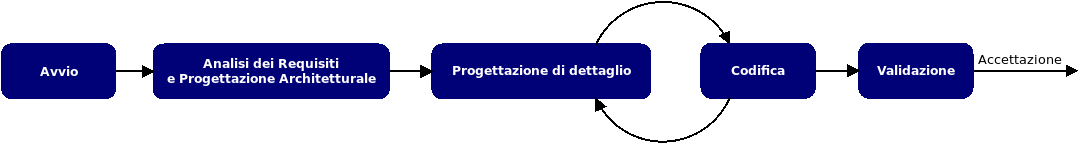
\includegraphics[scale=0.4]{images/Model/model.png}
	\caption{Ciclo di vita}
\end{figure}

\subsection{Attività}
Ogni incremento prevede delle attività. Ognuna di esse viene assegnata dal responsabile a uno dei membri del team di sviluppo, il quale svolgerà il lavoro assegnato. Una volta completato, il lavoro dovrà essere sottoposto a verifica.\\
Nel caso in cui il risultato sia soddisfacente, l'attività è considerata conclusa e il responsabile potrà assegnarne una nuova al membro.\\ 
In caso contrario, il lavoro non è considerato completato e lo sviluppatore dovrà correggere dove indicato durante l'incremento successivo. Le correzioni effettuate dovranno essere a loro volta verificate.\\
La quantità di giorni lavorativi per ciascuna attività varia dai 5 ai 10 giorni dipendentemente dalla sua complessità.

\begin{figure}[h]
	\centering
	
\includegraphics[scale=0.45]{images/Model/activity.png}
	\caption{Ciclo di un'attività}
\end{figure}

		\newpage	

	\section{Pianificazione}
		Per la pianificazione, sono stati individuati 5 periodi, scelti in base ai processi primari coinvolti. Ogni periodo contiene diverse attività. Nella pianificazione, verrà impiegata tale numerazione:
\begin{center}
	[\textbf{Periodo}].[\textbf{Attività}]
\end{center}
se le attività non vengono raggruppate,
\begin{center}
	[\textbf{Periodo}].[\textbf{Insieme di attività}].[\textbf{Attività}]
\end{center}
altrimenti.\\
La numerazione, sia per i periodi, sia per gli insiemi di attività, sia per le singole attività, è sequenziale.\\
Alla fine di ogni periodo, segue la tabella con le assegnazioni dei membri alle attività. Nella prima colonna di ogni tabella, si trovano le attività, indicate col numero assegnato. Nelle restanti, viene indicato a quale membro è stata affidata ciascuna attività tramite un $\bullet$ nella relativa colonna. I nominativi dei membri sono stati sostituiti con le prime tre lettere del cognome: BER (Bergo), BOR (Bortone), COS (Cosentino), MAR (Marcato), PEA (Peagno), PER (Peron), PET (Pettenuzzo).

\newpage
\subsection{Periodo di Avvio e di Analisi (2018-12-04 - 2018-02-09)}
		\subsubsection{Periodo di Avvio (2018-12-04 - 2018-12-17)}
		Nel periodo di avvio hanno luogo le seguenti attività:
		\begin{enumerate}[label = 1.\arabic*)]
			\item ricerca degli strumenti (2018-12-4 - 2018-12-14): tutti i membri del gruppo effettuano le ricerche sui possibili strumenti utili alle attività di avvio e di analisi dei requisiti;
			\item prima normazione (2018-12-5 - 2018-12-14): gli amministratori redigono le \textit{Norme di progetto} concordate per i processi di supporto e organizzativi;
			\item studio di fattibilità (2018-12-4 - 2018-12-8): gli analisti effettuano lo \textit{Studio di fattibilità} dei capitolati;
			\item pianificazione di progetto (2018-12-7 - 2018-12-13): il responsabile redige il \textit{Piano di progetto}, riportando modello di sviluppo, analisi dei rischi e la pianificazione per le prime attività dell'analisi dei requisiti;
			\item verifica dei documenti (2018-12-15 - 2018-12-16): i verificatori controllano se i documenti siano corretti.
		\end{enumerate}
		
	\subsubsection{Periodo di Analisi (2018-12-17 - 2018-02-09)}	
		\paragraph{Pianificazione (2018-12-17 - 2018-12-23)\\} Il periodo di analisi dei requisiti inizia con le attività di:
			\begin{enumerate}[label = 2.1.\arabic*)]
				\item pianificazione di progetto (2018-12-17 - 2018-12-21): il responsabile effettua il resoconto del periodo di avvio e pianifica in maniera più dettagliata le attività di analisi dei requisiti; 
				\item pianificazione della qualifica (2018-12-17 - 2018-12-21): i verificatori redigono il resoconto del periodo di avvio e gli amministratori effettuano i primi incrementi per il \textit{Piano di qualifica};
				\item normazione (2018-12-17 - 2018-12-21): gli amministratori redigono in maniera precisa e completa le \textit{Norme di progetto} per l'attività di analisi;
				\item verifica del \textit{Piano di progetto}, del \textit{Piano di qualifica} e delle \textit{Norme di progetto} (2018-12-21 - 2018-12-23).
			\end{enumerate}
		\paragraph{Analisi dei requisiti (2018-12-19 - 2018-02-09)\\} La parte centrale del periodo di analisi dei requisiti è costituita dalle attività di:
			\begin{enumerate}[label = 2.2.\arabic*)]
				\item analisi dei requisiti del sistema (2018-12-19 - 2018-12-27): gli analisti svolgono la prima analisi dei requisiti del sistema;
				\item incrementi al \textit{Piano di qualifica} (2018-12-26 - 2018-12-30): gli analisti introducono nel piano i test di sistema in base a quanto scaturito dall'analisi dei requisiti;
				\item verifica dell'analisi dei requisiti di sistema (2018-12-29 - 2018-12-31)
				\item verifica del \textit{Piano di qualifica} (2018-01-09 - 2019-01-03)
				\item incrementi all'analisi dei requisiti (2019-01-02 - 2019-01-08): gli analisti aggiungono degli incrementi all'analisi di sistema
				\item verifica degli incrementi all'analisi dei requisiti (2019-01-09 - 2019-01-11)
				\item incrementi al \textit{Piano di progetto} (2019-01-07 - 2019-01-10): il responsabile redige la parte di rendicontazione e consuntivo del \textit{Piano di progetto} da presentare alla Revisione dei Requisiti.
				\item incrementi al \textit{Piano di qualifica} (2019-01-07 - 2019-01-10): i verificatori redigono la parte di rendicontazione del \textit{Piano di qualifica} da presentare alla Revisione dei Requisiti, aggiungendo i risultati delle misurazioni effettuate, e gli analisti aggiungono i restanti test di sistema.
				\item verifica del \textit{Piano di progetto} e del \textit{Piano di qualifica} (2019-01-11 - 2019-01-12)
				\item preparazione alla presentazione (2019-01-15 - 2019-01-20);
				\item analisi dei requisiti software (2019-02-01 - 2019-02-05): gli analisti effettuano l'analisi dei requisiti software. Quest'attività è successiva al primo incremento di progettazione architetturale.
				\item verifica dell'analisi dei requisiti (2019-02-07 - 2019-02-09)				
			\end{enumerate}

	\begin{table}[h]
		\caption{Tabella delle assegnazioni per il periodo di avvio}
		\centering		
		\begin{tabular}{| >{\centering}p{1.5cm} | c | c | c | c | c | c | c |}
			\rowcolor{LightBlue}
			\textbf{\color{white}Numero attività} 
			& \textbf{\color{white}BER} 
			& \textbf{\color{white}BOR} 
			& \textbf{\color{white}COS} 
			& \textbf{\color{white}MAR} 
			& \textbf{\color{white}PEA} 
			& \textbf{\color{white}PER} 
			& \textbf{\color{white}PET}\\

			1.1 & $\bullet$ & $\bullet$ & $\bullet$ & $\bullet$ & $\bullet$ & $\bullet$ & $\bullet$ \\
			\rowcolor{LightGray}
			1.2 & $\bullet$ &   &   & $\bullet$ & $\bullet$ &   & $\bullet$ \\
			1.3 & $\bullet$ &   & $\bullet$ & $\bullet$ & $\bullet$ & $\bullet$ & $\bullet$ \\ 
			\rowcolor{LightGray}
			1.4 &   &   & $\bullet$ &   &   &   &   \\ 
			1.5 &   & $\bullet$ &   &   & $\bullet$ & $\bullet$ &   \\ \hline
		\end{tabular}
	\end{table}

	\begin{table}[h]
		\caption{Tabella delle assegnazioni per il periodo di analisi}
		\centering
		\begin{tabular}{| >{\centering}p{1.5cm} | c | c | c | c | c | c | c |}
			\rowcolor{LightBlue}
			\textbf{\color{white}Numero attività} 
			& \textbf{\color{white}BER} 
			& \textbf{\color{white}BOR} 
			& \textbf{\color{white}COS} 
			& \textbf{\color{white}MAR} 
			& \textbf{\color{white}PEA} 
			& \textbf{\color{white}PER} 
			& \textbf{\color{white}PET}\\
		
			2.1.1  &   &   & $\bullet$ & $\bullet$ &   &   &   \\
			\rowcolor{LightGray}	
			2.1.2  &   & $\bullet$ &   &   &   & $\bullet$ &   \\
			2.1.3  & $\bullet$ &   &   &   & $\bullet$ &   & $\bullet$ \\
			\rowcolor{LightGray}
			2.1.4  & $\bullet$ & $\bullet$ &   &   &   & $\bullet$ &   \\
			2.2.1  &   &   & $\bullet$ & $\bullet$ & $\bullet$ & $\bullet$ &   \\
			\rowcolor{LightGray}
			2.2.2  &   &   &   & $\bullet$ & $\bullet$ & $\bullet$ &   \\
			2.2.3  & $\bullet$ & $\bullet$ &   &   &   &   & $\bullet$ \\
			\rowcolor{LightGray}
			2.2.4  &   &   & $\bullet$ &   &   &   & $\bullet$ \\
			2.2.5  & $\bullet$ & $\bullet$ &   &   &   & $\bullet$ & $\bullet$ \\
			\rowcolor{LightGray}
			2.2.6  &   &   & $\bullet$ & $\bullet$ & $\bullet$ &   &   \\
			2.2.7  &   &   &   &   & $\bullet$ &   &   \\
			\rowcolor{LightGray}
			2.2.8  &   &   & $\bullet$ & $\bullet$ &   &   &   \\
			2.2.9  & $\bullet$ &   &   &   &   &   & $\bullet$ \\
			\rowcolor{LightGray}
			2.2.10 & $\bullet$ & $\bullet$ & $\bullet$ & $\bullet$ & $\bullet$ & $\bullet$ & $\bullet$ \\
			2.2.11 & $\bullet$ & $\bullet$ & $\bullet$ &   &   &   &   \\
			\rowcolor{LightGray}
			2.2.12 &   &   &   & $\bullet$ & $\bullet$ &   &   \\ \hline
		\end{tabular}
	\end{table}
	


\newpage
\subsection{Periodo di Progettazione (2018-12-22 - 2019-04-21)}	
	\subsubsection{Pianificazione (2019-01-22 - 2019-01-03)\\} 
			\begin{enumerate}[label = 3.1.\arabic*)]
				\item Ricerca delle tecnologie (2018-01-22 - 2018-01-28);
				\item Normazione (2018-01-22 - 2018-01-25);
				\item Incrementi \textit{Piano di progetto} (2018-01-22 - 2018-01-25);
				\item Incrementi \textit{Piano di qualifica} (2018-01-22 - 2018-01-25);
				\item Verifica degli incrementi delle \textit{Norme di progetto}, del \textit{Piano di progetto} e del \textit{Piano di qualifica} (2018-01-27 - 2018-01-29).
			\end{enumerate}
	
		\subsubsection{Progettazione architetturale (2018-01-26 - 2018-02-16)\\} La parte centrale della progettazione sono le attività di:
			\begin{enumerate}[label = 3.2.\arabic*)]
				\item Progettazione architetturale (2018-01-26 - 2018-01-31): i progettisti stilano il documento \textit{Technology baseline} contenente scelte progettuali ad alto livello;
				\item Verifica progettazione architetturale (2018-02-04 - 2018-02-06);
				\item Incrementi di progettazione architetturale (2018-02-06 - 2018-02-12);
				\item Verifica degli incrementi della Progettazione architetturale (2018-02-14 - 2018-02-16);
			\end{enumerate}

		\subsubsection{Progettazione di dettaglio (2019-02-14 - 2019-03-01)\\} La parte che conclude la Progettazione sono le attività di:
			\begin{enumerate}[label = 3.3.\arabic*)]
				\item Progettazione di dettaglio(2019-02-14 - 2019-02-20): i progettisti redigono il documento \textit{Product baseline} contenente i dettagli della progettazione architetturale definita in \textit{Technology baseline};
				\item Verifica progettazione di dettaglio (2019-02-22 - 2019-02-23);
				\item Incrementi di progettazione di dettaglio(2019-02-28 - 2019-03-04);
				\item Verifica progettazione di dettaglio (2019-03-05 - 2019-03-06);
				\item Incrementi \textit{Piano di progetto} (2019-02-27 - 2019-03-01);
				\item Incrementi \textit{Piano di qualifica} (2019-02-27 - 2019-03-01);	
				\item Verifica degli incrementi del \textit{Piano di progetto} e del \textit{Piano di qualifica} (2019-03-03 - 2019-03-04);
				\item Preparazione della presentazione (2019-03-09 - 2019-03-14);
				\item Incrementi di Progettazione di dettaglio (2019-03-24 - 2019-03-28);
				\item Verifica degli incrementi di progettazione di dettaglio (2019-03-29 - 2019-03-30);
				\item Incrementi di Progettazione di dettaglio (2019-04-15 - 2019-04-19);
				\item Verifica incrementi di Progettazione di dettaglio (2019-04-20 - 2019-04-21).
			\end{enumerate}
	
	\begin{table}[h]
		\caption{Tabella delle assegnazioni per il periodo di progettazione}
		\centering		
		\begin{tabular}{| >{\centering}p{1.5cm} | c | c | c | c | c | c | c |}
			\rowcolor{LightBlue}
			\textbf{\color{white}Numero attività} 
			& \textbf{\color{white}BER} 
			& \textbf{\color{white}BOR} 
			& \textbf{\color{white}COS} 
			& \textbf{\color{white}MAR} 
			& \textbf{\color{white}PEA} 
			& \textbf{\color{white}PER} 
			& \textbf{\color{white}PET}\\

			3.1.1 & $\bullet$ &	& $\bullet$ &	&	&	&	\\
			\rowcolor{LightGray}
			3.1.2 &	& $\bullet$ &   &	&	&   &	\\
			3.1.3 &	&   &	& $\bullet$ &	& $\bullet$ &	\\ 
			\rowcolor{LightGray}
			3.1.4 &   &   &	&  & $\bullet$ &   & $\bullet$ \\ 
			3.1.5 &   & $\bullet$ &   &  & $\bullet$ &	&   \\ 
			\rowcolor{LightGray}
			3.2.1 &   &   &	& $\bullet$ &   & $\bullet$ & $\bullet$ \\ 
			3.2.2 &   & $\bullet$ &   &   & $\bullet$ &	&  \\
			\rowcolor{LightGray}
			3.2.3 & $\bullet$ & $\bullet$ & $\bullet$ &   &   &   & $\bullet$  \\ 
			3.2.4 &	  &   &  & $\bullet$ & $\bullet$ &   &   \\
			\rowcolor{LightGray}
			3.3.1 & $\bullet$  & $\bullet$ & $\bullet$  &  &  & $\bullet$	&  \\
			3.3.2 &   & $\bullet$  &   & $\bullet$  &  &	&  \\
			\rowcolor{LightGray}
			3.3.3 &   &  & $\bullet$  &   &  & $\bullet$ &  \\
			3.3.4 &   &  &   & $\bullet$  &  &	&  \\
			\rowcolor{LightGray}
			3.3.5 & $\bullet$ &  &   &   &  &	&  \\
			3.3.6 &   & $\bullet$ &   &   &  &	&  \\
			\rowcolor{LightGray}
			3.3.7 &   &  &   &   &  &$\bullet$	& $\bullet$  \\
			3.3.8 & $\bullet$  & $\bullet$ & $\bullet$ & $\bullet$ & $\bullet$ & $\bullet$ & $\bullet$\\
			\rowcolor{LightGray}			
			3.3.9 &   & $\bullet$ &   &   & $\bullet$ & $\bullet$ &   \\
			3.3.10 &   &   &   & $\bullet$ &  & 	&   \\
			\rowcolor{LightGray}			
			3.3.11 &   & $\bullet$ & $\bullet$ &   &  & 	&   \\
			3.3.12 & $\bullet$ &  &   &   &  & 	&   \\
			\hline
		\end{tabular}
	\end{table}
	

	
\newpage	
\subsection{Periodo di Realizzazione (2019-02-21 - 2019-05-01)}
	Nella fase 3 hanno luogo le seguenti attività:
\begin{itemize}
	\item normazione: modifiche alle \textit{NormeDiProgetto\_v2.0.0} secondo quanto segnalato alla Revisione di progettazione. Si procede poi con il suo incremento;
	\item pianificazione della qualifica: modifiche al \textit{PianoDiQualifica\_v2.0.0} secondo quanto segnalato alla Revisione di Progettazione. Si procede poi con il suo incremento;
	\item pianificazione delle attività: modifiche al \textit{PianoDiProgetto\_v2.0.0} secondo quanto segnalato alla Revisione di progettazione;
	\item progettazione in dettaglio e Product Baseline: questa attività consiste nella progettazione del prodotto tramite diagrammi delle classi e di sequenza, incrementando quanto sviluppato nel PoC.
	\item codifica: realizzazione del prodotto;
	\item verifica per il colloquio: verifica del codice scritto in vista del colloquio Agile con il committente;
	\item colloquio: viene effettuato il colloquio con il committente;
	\item redazione manuali: redazione \textit{Manuale Utente} e \textit{Manuale Sviluppatore};
	\item incremento progettazione e codifica: in base alle segnalazioni ricevute al colloquio con il committente viene eseguito l'eventuale incremento;
	\item incremento della pianificazione delle attività: viene aggiornato il \textit{Piano di Progetto} con il consuntivo pre-finale;
	\item verifica per la consegna: vengono verificati tutti i documenti e il Product Baseline con la relativa codifica;
	\item approvazione dei documenti da parte del responsabile. Sono pronti per il rilascio le \textit{NormeDiProgetto\_v3.0.0}, il \textit{PianoDiProgetto\_v3.0.0}, il \textit{PianoDiQualifica\_v3.0.0}, l'\textit{AnalisiDeiRequisiti\_v3.0.0}, il
	\textit{ManualeUtente\_v1.0.0} e il \textit{ManualeSviluppatore\_v1.0.0}
	\item preparazione alla presentazione.
\end{itemize}

\begin{tabularx}{\textwidth}{| c | c | c | }
		\rowcolor{LightBlue}
		\color{white}\bfseries Incremento 1 & 
		\color{white}\bfseries Incremento 2 & 
		\color{white}\bfseries Incremento 3 \\[0.25cm]
		ROF1 & ROF7 & ROF22 \\ 
		ROF2 & ROF8 & ROF27 \\ 
		ROF3 & ROF9 & ROF28 \\ 
		ROF4 & ROF10 & ROF29 \\ 
		ROF5 & ROF11 & ROF30 \\ 
		ROF6 & ROF12 & ROF31 \\ 
		ROF23 & ROF13 & ROF32 \\ 
		ROF24 & ROF14 & ROF33 \\ 
		ROF25 & ROF15 & ROF34 \\ 
		ROF26 & ROF16 & ROF35 \\ 
		ROF33 & ROF17 & ROF36 \\ 
		& ROF18 & ROF37 \\ 
		& ROF19 & \\ 
		& ROF20 & \\ 
		& ROF21 & \\ 
		& RDF1 & \\ 
		& RDF2 & \\ 
		& RDF9 & \\ \hline
	\end{tabularx}

\begin{figure}[h]
	\centering
	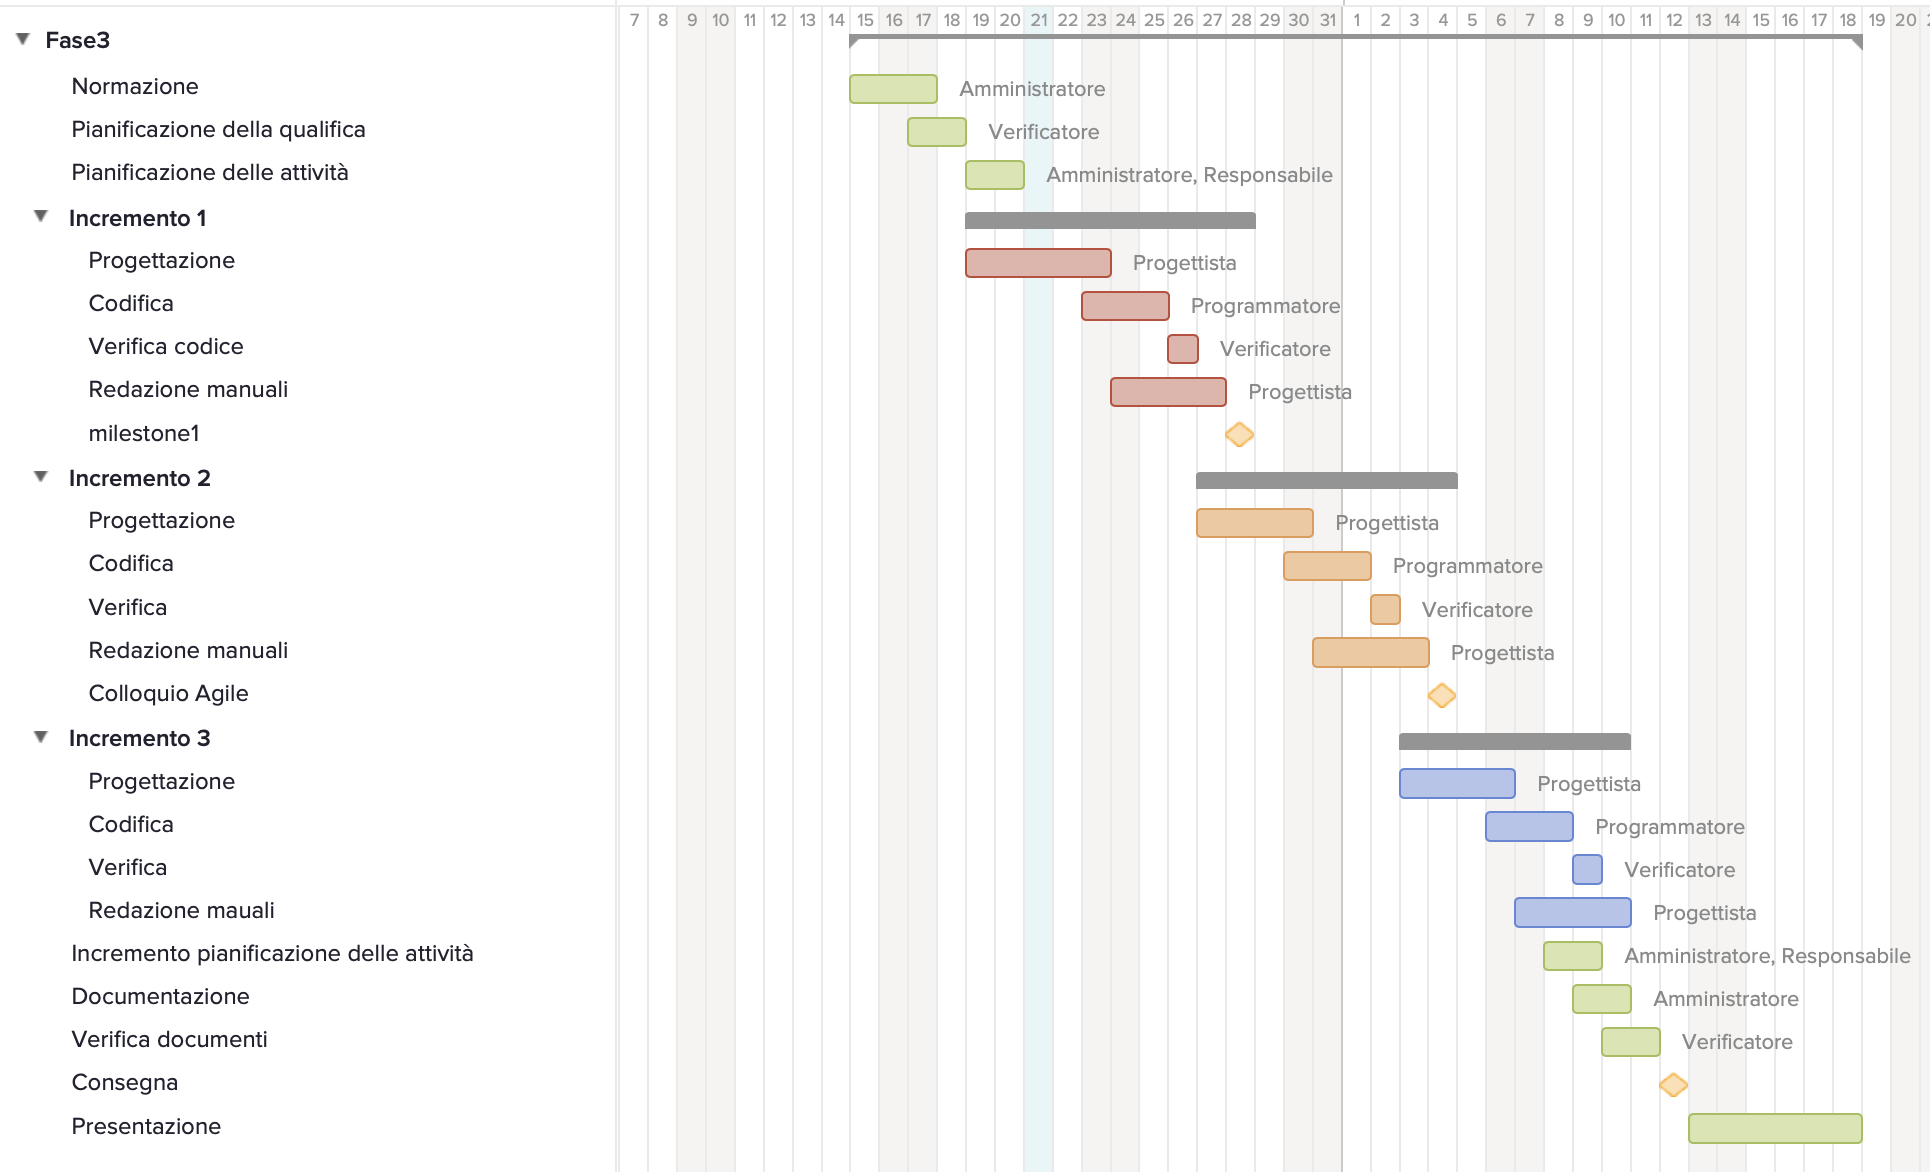
\includegraphics[scale=0.70]{images/fase3.png}
	\caption{Diagramma di Gantt riguardante la fase 3}
\end{figure}
	
\newpage	
\subsection{Periodo di Validazione (2019-04-13 - 2019-05-12)}
	Nella fase 4 vengono eseguiti i seguenti incrementi e attività:
\begin{itemize}
	\item Incremento 1
			\begin{itemize}
				\item normazione: modifiche alle \textit{NormeDiProgetto\_v3.0.0} secondo quanto segnalato alla Revisione di Qualifica. Si procede poi con il suo incremento;
				\item pianificazione della qualifica: modifiche al \textit{PianoDiQualifica\_v3.0.0} secondo quanto segnalato alla Revisione di qualifica. Si procede poi con il suo incremento;
				\item pianificazione delle attività: modifiche al \textit{PianoDiProgetto\_v3.0.0} secondo quanto segnalato alla Revisione di Qualifica;
			\end{itemize}
	\item Incremento 2 e Incremento 3
		\begin{itemize}
			\item progettazione di dettaglio: incremento al \textit{Product Baseline} con i requisiti indicati nella tabella 4;
			\item codifica: codifica degli incrementi effettuati durante la progettazione;
			\item redazione manuali: incrementi al \textit{ManualeUtente\_v1.0.0} e al \textit{ManualeSviluppatore\_v1.0.0} in base a quanto segnalato alla Revisione di Qualifica;
			\item verifica: verifica degli incrementi effettuati;
		\end{itemize}
	\item Incremento 4
		\begin{itemize}
			\item Documentazione;
			\item Verifica documentazione;
		\end{itemize}
	\item validazione e collaudo: vengono eseguiti i test di qualifica e il collaudo per il rilascio;
	\item preparazione alla presentazione;
	\item approvazione dei documenti da parte del responsabile. Sono pronti per il rilascio le \textit{NormeDiProgetto\_v4.0.0}, il \textit{PianoDiProgetto\_v4.0.0}, il \textit{PianoDiQualifica\_v4.0.0}, l'\textit{AnalisiDeiRequisiti\_v4.0.0} il
	\textit{ManualeUtente\_v2.0.0} e il \textit{ManualeSviluppatore\_v2.0.0};
\end{itemize}

\begin{tabularx}{\textwidth}{| c | c | }
	\rowcolor{LightBlue}
	\color{white}\bfseries Incremento 1 & 
	\color{white}\bfseries Incremento 2  \\[0.25cm]
	RDF22 & RDF3 \\ 
	RDF23 & RDF4 \\ 
	RDF24 & RDF5 \\ 
	RDF25 & RDF6 \\ 
	RDF26 & RDF7 \\ 
	RDF27 & RDF8 \\ 
	RDF28 & RDF10 \\ 
	RDF29 & RDF11 \\ 
	RDF30 & RDF12 \\ 
	RDF31 & RDF13 \\ 
	RDF32 & RDF14 \\ 
	RDF33 & RDF15 \\ 
	RDF34 & RDF16 \\ 
	RDF35 & RDF17 \\ 
	RDF36 & RDF18 \\
	RDF37 & RDF19\\
	RDF38 & RDF20 \\
	RDF39 & RDF21 \\
	RDF40 &  \\
	RDF41 &  \\
	RDF42 &  \\
	RDF43 &  \\
	RDF44 &  \\
		 \hline
		 \caption{Requisiti da soddisfare in fase 4}
\end{tabularx}

\begin{figure}[h]
	\centering
	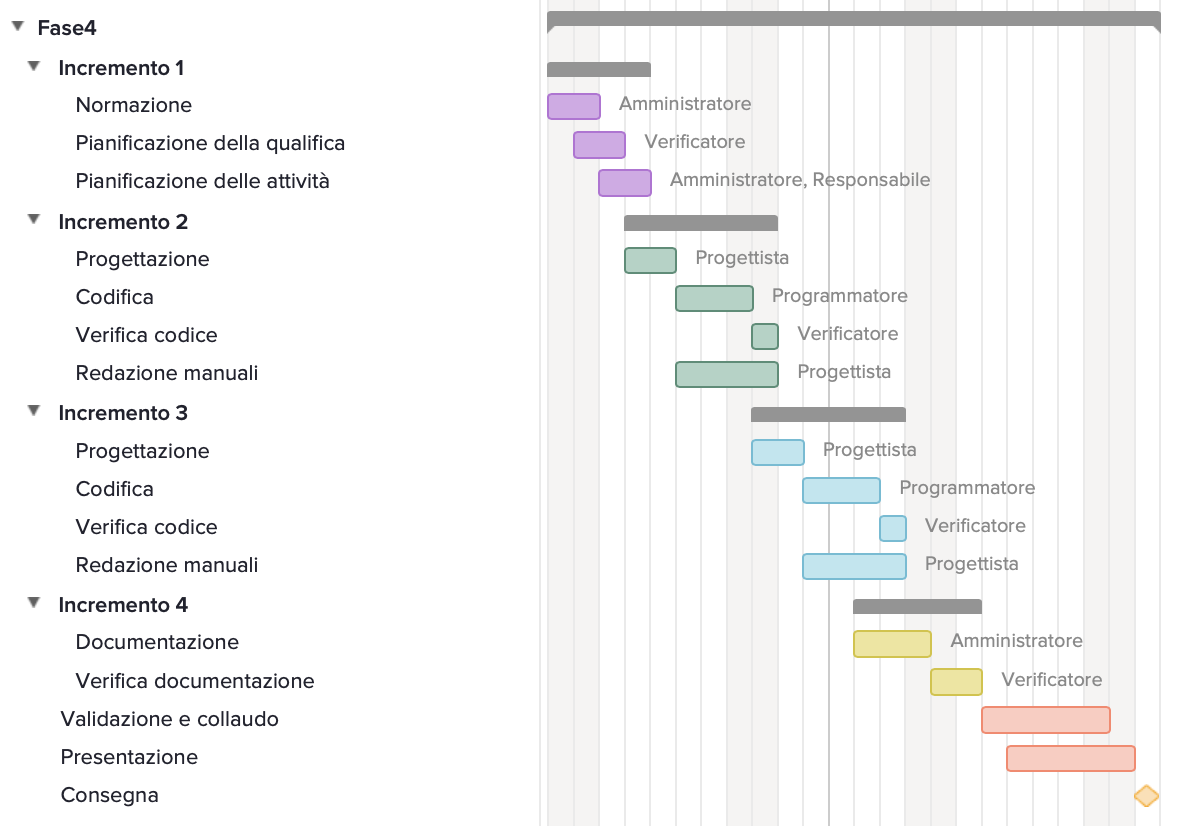
\includegraphics[scale=0.70]{images/fase4.png}
	\caption{Diagramma di Gantt riguardante la fase 4}
\end{figure}
	
\newpage
\subsection{Diagrammi di Gantt}
\begin{figure}[hbt!]
	\centering
	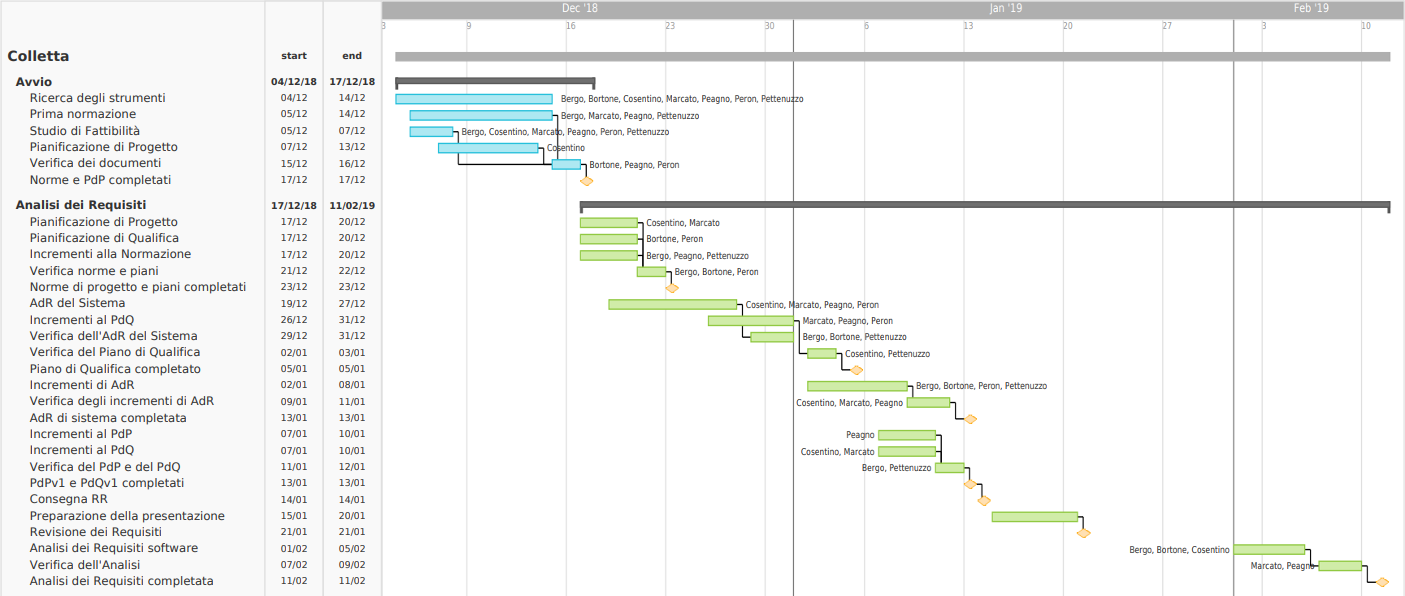
\includegraphics[scale=0.45,angle=90]{images/ganttan.png}
	\caption{Diagramma di Gantt per il periodo di avvio e di analisi}
\end{figure}

\newpage
\begin{figure}[hbt!]
	\centering
	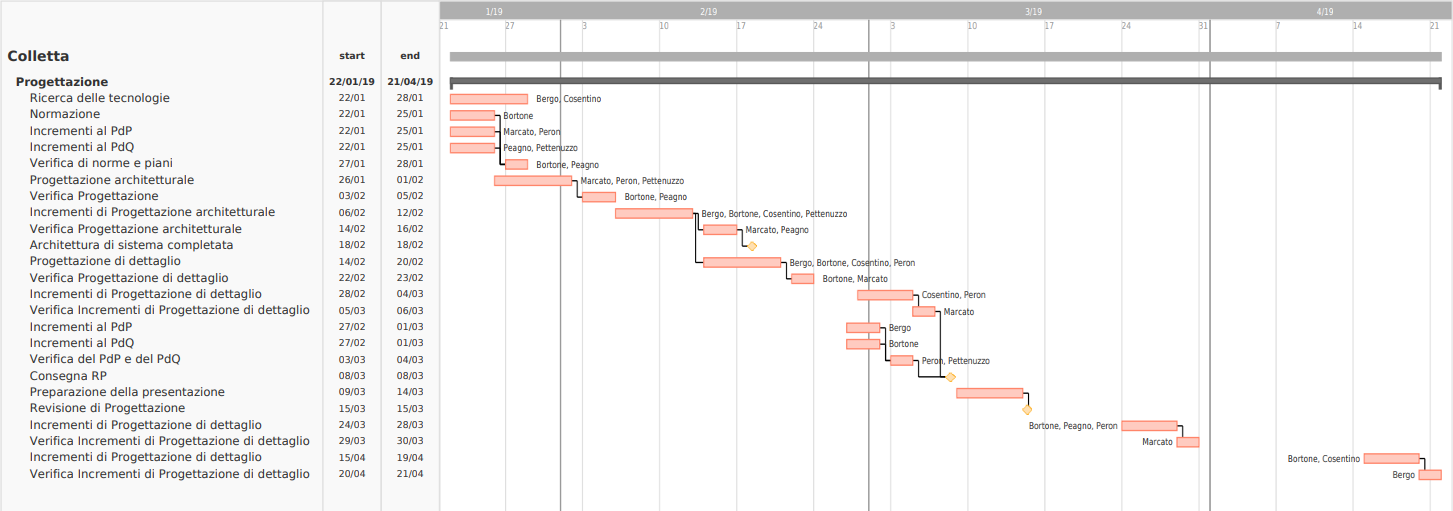
\includegraphics[scale=0.45,angle=90]{images/ganttprog.png}
	\caption{Diagramma di Gantt per il periodo progettazione}
\end{figure}

\newpage
\begin{figure}[hbt!]
	\centering
	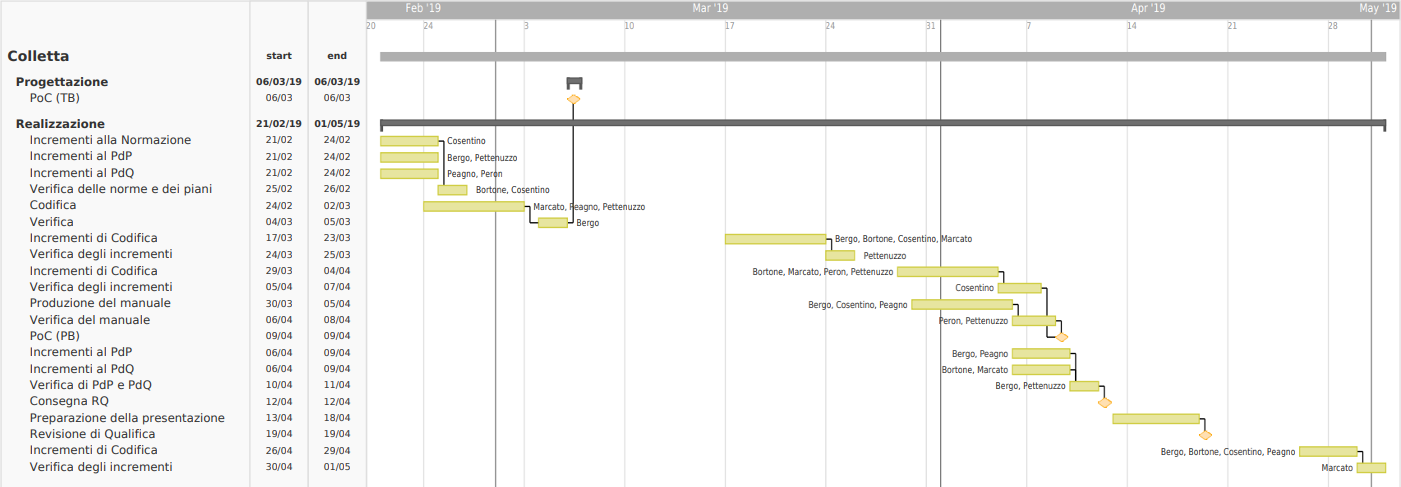
\includegraphics[scale=0.45, angle=90]{images/ganttreal.png}
	\caption{Diagramma di Gantt per il periodo di realizzazione}
\end{figure}

\newpage
\begin{figure}[hbt!]
	\centering
	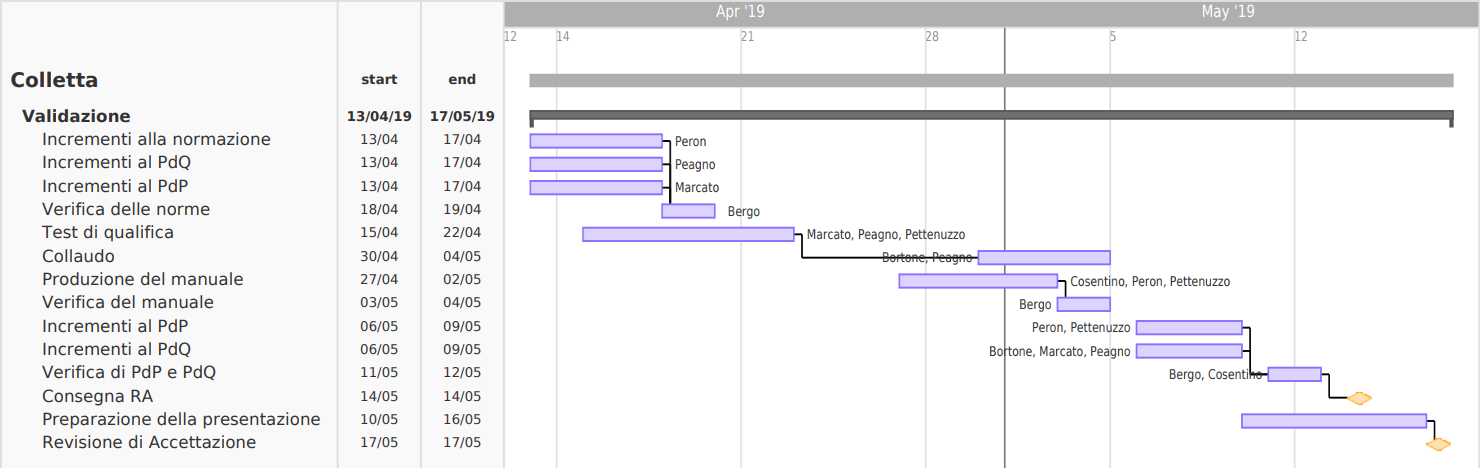
\includegraphics[scale=0.40, angle=90]{images/ganttval.png}
	\caption{Diagramma di Gantt per il periodo di validazione}
\end{figure}
		\newpage
				
	\section{Preventivo}
		In questa sezione, vengono riportati il preventivo per ogni periodo del progetto e i dati utili a ricavarlo. Il preventivo definisce il budget e quindi il costo totale del progetto. Ogni tabella fa riferimento a una specifica fase del progetto (indicata con un numero sequenziale) che parte da una determinata data a un'altra.
Le fasi individuate corrispondono agli intervalli tra una revisione e l'altra e, nel caso della fase 1, all'intervallo di tempo che parte dall'inizio del progetto fino alla Revisione dei Requisiti. In particolare,
\begin{enumerate}
	\item Fase 1 (2018-12-04 - 2019-01-21); 
	\item Fase 2 (2019-01-22 - 2019-03-15);
	\item Fase 3 (2019-03-16 - 2019-04-19);
	\item Fase 4 (2019-04-20 - 2019-05-17).
\end{enumerate}
Per ogni fase sono presenti: un prospetto orario che indica le ore preventivate per ciascun membro e per ciascun ruolo, una tabella dei costi per membro e una tabella dei costi per ruolo.\\
Per indicare i ruoli, sono state impiegate le seguenti abbreviazioni:
\begin{itemize}
	\item RES: responsabile;
	\item AMM: amministratore;
	\item AN: analista;
	\item PRO: progettista;
	\item DEV: programmatore;
	\item VER: verificatore.
\end{itemize}

\newpage
\subsection{Fase 1 (2018-12-04 - 2019-01-21)}
	Le ore di questo periodo vanno considerate come investimento e non rientrano nelle ore da rendicontare per il preventivo.
	\subsubsection{Ore preventivate}
		La seguente tabella indica le ore di lavoro per ciascun membro e per ciascun ruolo:
		\begin{table}[h]
			\centering
			\begin{tabular}{| l | c c c c c c | c |}
				\rowcolor{LightBlue}
				& \multicolumn{7}{c}{\textbf{\color{white}Numero di ore}}	\\
	
				\rowcolor{LightBlue}
				\textbf{\color{white}Membro}
				& \textbf{\color{white}RES}
				& \textbf{\color{white}AMM}
				& \textbf{\color{white}AN}
				& \textbf{\color{white}PRO}
				& \textbf{\color{white}DEV}
				& \textbf{\color{white}VER}
				& \textbf{\color{white}Totali}\\
	
				Bergo 				& - & 15 & 14 & - & - & 8 & 37\\
				Bortone 			& - & 10 & 15	& - & - & 8 & 33\\
				Cosentino 		& 20 & - & 22 & - & - & 5 & 47\\
				Marcato 			& 5 & 10 & 25 & - & - & 3 & 43\\
				Peagno 			& 5 & 15 & 22 & - & - & 3 & 45\\
				Peron 				& - & 10 & 29 & - & - & 5 & 44\\
				Pettenuzzo 	& - & 15 & 19 & - & - & 5 & 39\\ \hline
			\end{tabular}
			\caption{Ore di lavoro per membro/ruolo della fase 1}
		\end{table}
		
	\subsubsection{Costo}
		Le seguenti tabelle indicano i costi in base ai membri e in base ai ruoli:
		\begin{table}[h]
			\centering		
			\begin{tabular}{| l | l |}
				\rowcolor{LightBlue}
				\textbf{\color{white}Membro}
				& \textbf{\color{white}Costo}\\
			
				Bergo 				& 770€\\
				Bortone 			& 695€\\
				Cosentino 		& 1225€\\
				Marcato 			& 1020€\\
				Peagno 			& 1045€\\
				Peron 				& 1000€\\
				Pettenuzzo 	& 850€\\ \hline
				\textbf{Totale} & 6605€\\ \hline
			\end{tabular}
			\caption{Costo di ciascun membro nella fase 1}
		\end{table}
		
		\begin{table}[h]
			\centering		
			\begin{tabular}{| l | l |}
				\rowcolor{LightBlue}
				\textbf{\color{white}Ruolo}
				& \textbf{\color{white}Costo}\\
			
				Responsabile 		& 900€\\
				Amministratore 	& 1500€\\
				Analista 				& 3650€\\			
				Progettista 			& 0€\\
				Programmatore 		& 0€\\
				Verificatore 		& 555€\\ \hline
				\textbf{Totale} 	& 6605€\\ \hline
			\end{tabular}
			\caption{Costo di ciascun ruolo nella fase 1}
		\end{table}

\newpage
\subsection{Fase 2 (2019-01-22 - 2019-03-15)}
	\subsubsection{Ore preventivate}
		La seguente tabella indica le ore di lavoro per ciascun membro e per ciascun ruolo:
		\begin{table}[h]
			\centering
			\begin{tabular}{| l | c c c c c c | c |}
				\rowcolor{LightBlue}
				& \multicolumn{7}{c}{\textbf{\color{white}Numero di ore}}	\\
	
				\rowcolor{LightBlue}
				\textbf{\color{white}Membro}
				& \textbf{\color{white}RES}
				& \textbf{\color{white}AMM}
				& \textbf{\color{white}AN}
				& \textbf{\color{white}PRO}
				& \textbf{\color{white}DEV}
				& \textbf{\color{white}VER}
				& \textbf{\color{white}Totali}\\

				Bergo      & 10 & - & 10 & 25 & - & 2 	& 47 \\
				Bortone    & - & 5 & 10 & 30 & - & 7 & 52 \\
				Cosentino  & - & 5 & 10 & 30 & - & 2 & 47 \\
				Marcato    & 5 & - & - & 15 & 15 & 8 & 43 \\
				Peagno     & - & - & - & 10 & 25 & 10 & 45 \\
				Peron      & 5 & - & - & 50 & - & 3 & 58 \\
				Pettenuzzo & 5 & - & - & 30 & 15 & 3 & 53 \\ \hline
			\end{tabular}
			\caption{Ore di lavoro per membro/ruolo della fase 2}
		\end{table}		
		
	\subsubsection{Costo}
		Le seguenti tabelle indicano i costi in base ai membri e in base ai ruoli:	
		\begin{table}[h]
			\centering
			\begin{tabular}{| l | l |}
				\rowcolor{LightBlue}
				\textbf{\color{white}Membro}
				& \textbf{\color{white}Costo}\\
			
				Bergo				& 1130€\\
				Bortone			& 1115€\\
				Cosentino		& 1040€\\
				Marcato			& 825€\\
				Peagno				& 745€\\
				Peron				& 1295€\\
				Pettenuzzo		& 1080€\\ \hline
				\textbf{Totale} & 7230€\\ \hline
			\end{tabular}
			\caption{Costo di ciascun membro nella fase 2}
		\end{table}
		
		\begin{table}[h]
			\centering
			\begin{tabular}{| l | l |}
				\rowcolor{LightBlue}
				\textbf{\color{white}Ruolo}
				& \textbf{\color{white}Costo}\\
			
				Responsabile 		& 750€\\
				Amministratore 	& 200€\\
				Analista 				& 750€\\			
				Progettista 			& 4180€\\
				Programmatore 		& 825€\\
				Verificatore 		& 525€\\ \hline
				\textbf{Totale} 	& 7230€\\ \hline
			\end{tabular}		
			\caption{Costo di ciascun ruolo nella fase 2}
		\end{table}
		
\newpage
\subsection{Fase 3 (2019-03-16 - 2019-04-19)}
	\subsubsection{Ore preventivate}
		La seguente tabella indica le ore di lavoro per ciascun membro e per ciascun ruolo:
		\begin{table}[h]
			\centering
			\begin{tabular}{| l | c c c c c c | c |}
				\rowcolor{LightBlue}
				& \multicolumn{7}{c}{\textbf{\color{white}Numero di ore}}	\\
	
				\rowcolor{LightBlue}
				\textbf{\color{white}Membro}
				& \textbf{\color{white}RES}
				& \textbf{\color{white}AMM}
				& \textbf{\color{white}AN}
				& \textbf{\color{white}PRO}
				& \textbf{\color{white}DEV}
				& \textbf{\color{white}VER}
				& \textbf{\color{white}Totali}\\
	
				Bergo      & 5 & - & - & 10 & 15 & 10 & 40 \\
				Bortone    & - & - & - & 15 & 20 & - & 35  \\
				Cosentino  & - & - & - & 15 & 15 & 3 & 33 \\
				Marcato    & 5 & - & - & 5 & 30 & 3 & 43 \\
				Peagno     & 5 & - & - & 30 & - & - & 35 \\
				Peron      & - & 5 & - & 10 & 15 & 2 & 32 \\
				Pettenuzzo & - & - & - & - & 15 & 15 & 30 \\ \hline
			\end{tabular}
			\caption{Ore di lavoro per membro/ruolo della fase 3}
		\end{table}
		
	\subsubsection{Costo}
		Le seguenti tabelle indicano i costi in base ai membri e in base ai ruoli:
		\begin{table}[h]
			\centering
			\begin{tabular}{| l | l |}
				\rowcolor{LightBlue}
				\textbf{\color{white}Membro}
				& \textbf{\color{white}Costo}\\
				
				Bergo 				& 745€\\
				Bortone 			& 630€\\
				Cosentino 		& 600€\\
				Marcato 			& 755€\\
				Peagno 			& 810€\\
				Peron 				& 575€\\
				Pettenuzzo 	& 450€\\ \hline
				\textbf{Totale} & 4565€\\ \hline
			\end{tabular}
			\caption{Costo di ciascun membro nella fase 3}
		\end{table}
		
		\begin{table}[h]
			\centering
			\begin{tabular}{| l | l |}
				\rowcolor{LightBlue}
				\textbf{\color{white}Ruolo}
				& \textbf{\color{white}Costo}\\
				
				Responsabile 		& 450€\\
				Amministratore 	& 100€\\
				Analista 				& 0€\\			
				Progettista 			& 1870€\\
				Programmatore 		& 1650€\\
				Verificatore 		& 495€\\ \hline
				\textbf{Totale} 	& 4565€\\ \hline
			\end{tabular}
			\caption{Costo di ciascun ruolo nella fase 3}
		\end{table}
		
\newpage
\subsection{Fase 4 (2019-04-20 - 2019-05-17)}
	\subsubsection{Ore preventivate}
		La seguente tabella indica le ore di lavoro per ciascun membro e per ciascun ruolo:
		\begin{table}[h]
			\centering
			\begin{tabular}{| l | c c c c c c | c |}
				\rowcolor{LightBlue}
				& \multicolumn{7}{c}{\textbf{\color{white}Numero di ore}}	\\
		
				\rowcolor{LightBlue}
				\textbf{\color{white}Membro}
				& \textbf{\color{white}RES}
				& \textbf{\color{white}AMM}
				& \textbf{\color{white}AN}
				& \textbf{\color{white}PRO}
				& \textbf{\color{white}DEV}
				& \textbf{\color{white}VER}
				& \textbf{\color{white}Totali}\\
	
				Bergo      & - & - & - & - & 10 & 5 & 15\\
				Bortone    & - & - & - & - & 10 & 7 & 17\\
				Cosentino  & - & - & - & 10 & 10 & 2 & 22\\
				Marcato    & - & - & - & - & - & 15 & 15\\
				Peagno     & - & - & - & - & 10 & 15 & 25\\
				Peron      & 5 & - & - & 10 & - & - & 15\\
				Pettenuzzo & 5 & - & - & 10 & - & 5 & 20\\ \hline
			\end{tabular}
			\caption{Ore di lavoro per membro/ruolo della fase 4}
		\end{table}
		
	\subsubsection{Costo}
		Le seguenti tabelle indicano i costi in base ai membri e in base ai ruoli:
		\begin{table}[h]
			\centering
			\begin{tabular}{| l | l |}
				\rowcolor{LightBlue}
				\textbf{\color{white}Membro}
				& \textbf{\color{white}Costo}\\
				
				Bergo				& 225€\\
				Bortone			& 255€\\
				Cosentino		& 400€\\
				Marcato			& 225€\\
				Peagno				& 375€\\
				Peron				& 370€\\
				Pettenuzzo		& 445€\\ \hline
				\textbf{Totale} & 2295€\\ \hline
			\end{tabular}
			\caption{Costo di ciascun membro nella fase 4}
		\end{table}
		
		\begin{table}[h]
			\centering
			\begin{tabular}{| l | l |}
				\rowcolor{LightBlue}
				\textbf{\color{white}Ruolo}
				& \textbf{\color{white}Costo}\\
				
				Responsabile 		& 300€\\
				Amministratore 	& 0€\\
				Analista 				& 0€\\			
				Progettista 			& 660€\\
				Programmatore 		& 600€\\
				Verificatore 		& 735€\\ \hline
				\textbf{Totale} 	& 2295€\\ \hline
			\end{tabular}		
			\caption{Costo di ciascun ruolo nella fase 4}
		\end{table}

\newpage
\subsection{Riepilogo}
	\subsubsection{Ore totali}
		La seguente tabella indica le ore di lavoro per ciascun membro e per ciascun ruolo. Tra parentesi vengono indicate le ore totali considerando anche l'investimento. Le ore rendicontate sono quelle delle fasi 2, 3 e 4. La fase 1 è da considerare come investimento per il progetto.
		\begin{table}[h]
			\centering
			\begin{tabular}{| l | c c c c c c | c |}
				\rowcolor{LightBlue}
				& \multicolumn{7}{c}{\textbf{\color{white}Numero di ore}}	\\
		
				\rowcolor{LightBlue}
				\textbf{\color{white}Membro}
				& \textbf{\color{white}RES}
				& \textbf{\color{white}AMM}
				& \textbf{\color{white}AN}
				& \textbf{\color{white}PRO}
				& \textbf{\color{white}DEV}
				& \textbf{\color{white}VER}
				& \textbf{\color{white}Totali}\\
		
				Bergo 				& 15 (15) & 0 (15)		& 10 (24)	& 35 (35) & 25 (25) & 17 (25)	& 102 (139)\\
				Bortone 			& -  (0)  & 5 (15)		& 10	 (25)	& 45 (45) & 30 (30) & 14 (22)	& 104 (137)\\
				Cosentino 		& -  (20) & 5 (5)		& 10 (32)	& 55 (55) & 25 (25) & 7  (12)	& 102 (149)\\
				Marcato 			& 10 (15) & 0 (10)		& -  (25)	& 20 (20) & 45 (45) & 26 (29)	& 101 (144)\\
				Peagno 			& 5  (10) & 0 (15)		& -  (22)	& 40 (40) & 35 (35) & 25 (28)	& 105 (150)\\
				Peron 				& 10 (10) & 5 (15)		& -  (29)	& 70 (70) & 15 (15) & 5  (10)	& 105 (149)\\
				Pettenuzzo 	& 10 (10) & 0 (15) 	& -  (19)	& 40 (40) & 30 (30) & 23 (28)	& 103 (142)\\ \hline
			\end{tabular}
			\caption{Ore di lavoro per membro/ruolo di tutto il progetto}
		\end{table}
	
	\subsubsection{Costo totale}
		Le seguenti tabelle indicano i costi con e senza investimento in base ai membri e in base ai ruoli.
		\begin{table}[h]
			\centering
			\begin{tabular}{| l | l | l |}
				\rowcolor{LightBlue}
				\textbf{\color{white}Membro}
				& \textbf{\color{white}Costo con investimento}
				& \textbf{\color{white}Costo preventivato}\\
				
				Bergo				& 2870€ & 2100€\\
				Bortone			& 2695€ & 2000€\\
				Cosentino		& 3265€ & 2040€\\
				Marcato			& 2825€ & 1805€\\
				Peagno				& 2975€ & 1930€\\
				Peron				& 3240€ & 2240€\\
				Pettenuzzo		& 2825€ & 1975€\\ \hline
				\textbf{Totale} & 20695€ & 14090€\\ \hline
			\end{tabular}
			\caption{Costo di ciascun membro per tutto il progetto}
		\end{table}
		
		\begin{table}[h]
			\centering
			\begin{tabular}{| l | l | l |}
				\rowcolor{LightBlue}
				\textbf{\color{white}Ruolo}
				& \textbf{\color{white}Costo con investimento}
				& \textbf{\color{white}Costo preventivato}\\
				
				Responsabile 		& 2400€ & 1500€\\
				Amministratore 	& 1800€ & 300€\\
				Analista 				& 4400€ & 750€\\			
				Progettista 			& 6710€ & 6710€\\
				Programmatore 		& 3075€ & 3075€\\
				Verificatore 		& 2310€ & 1755€\\ \hline
				\textbf{Totale} 	& 20695€ & 14090€\\ \hline
			\end{tabular}		
			\caption{Costo di ciascun ruolo per tutto il progetto}
		\end{table}
		
		\paragraph{Conclusioni\\}
		Il costo totale del progetto con un investimento di 6605 è pari a \textbf{20695€}. Conseguentemente, il costo preventivato è \textbf{14090€}.
		\newpage
				
	\section{Consuntivo di periodo}
		\subsection{Fase 1 (2018-12-04 - 2019-01-21)}
	\subsubsection{Ore impiegate}
		La seguente tabella indica le ore impiegate durante la fase 1. Tra parentesi viene indicata la differenza tra ore preventivate e ore impiegate ($preventivo - consuntivo$): valori positivi indicano le ore risparmiate e valori negativi indicano le ore in eccesso.
		\begin{table}[h]
			\centering
		\begin{tabular}{| l | c c c c c c | c |}
			\rowcolor{LightBlue}
			& \multicolumn{7}{c}{\textbf{\color{white}Numero di ore}}	\\
	
			\rowcolor{LightBlue}
			\textbf{\color{white}Membro}
			& \textbf{\color{white}RES}
			& \textbf{\color{white}AMM}
			& \textbf{\color{white}AN}
			& \textbf{\color{white}PRO}
			& \textbf{\color{white}DEV}
			& \textbf{\color{white}VER}
			& \textbf{\color{white}Totali}\\
	
			Bergo     		& -  (0)		& 9  (+6) 	& 22 (-8) 		& - (0) & - (0) & 7  (+1) 	& 34\\
			Bortone   		& -  (0)		& 14 (-4) 	& 18 (-3) 		& - (0) & - (0) & 10 (-2)	& 38\\
			Cosentino 		& 25 (-5) 	& -  (0) 	& 24 (-2) 		& - (0) & - (0) & -  (+5)	& 45\\
			Marcato   		& 10 (-5) 	& 10 (0) 	& 22 (+3) 		& - (0) & - (0) & -  (+3)	& 38\\
			Peagno    		& -  (+5) 	& 15 (0) 	& 23 (-1) 		& - (0) & - (0) & -  (+3)	& 34\\
			Peron     		& -  (0)		& 13 (-3) 	& 23 (+6) 		& - (0) & - (0) & 13 (-8)	& 44\\
			Pettenuzzo 	& - (0) 		& 12 (+3) 	& 5  (+14) 	& - (0) & - (0) & 13 (-8)	& 27\\ \hline
		\end{tabular}
		\caption{Ore di lavoro impiegate per membro/ruolo della fase 1}
	\end{table}
	\subsubsection{Costo}
		Le seguenti tabelle indicano i costi della fase 1. Nell'ultima colonna vengono indicate le differenze tra costi previsti e costi effettivi ($previsto - effettivo$): valori positivi indicano i risparmi e valori negativi indicano le perdite.
		\begin{table}[h]
			\centering
		\begin{tabular}{| l | l | l |}
			\rowcolor{LightBlue}
			\textbf{\color{white}Membro}
			& \textbf{\color{white}Costo}
			& \textbf{\color{white}Differenza}\\
			
			Bergo 				& 835€ 	& -65€\\
			Bortone 			& 880€ 	& -185€\\
			Cosentino 		& 1350€ 	& -125€\\
			Marcato 			& 1050€ 	& -30€\\
			Peagno 			& 875€ 	& +170€\\
			Peron 				& 1030€ 	& -30€\\
			Pettenuzzo 	& 560€ 	& +290€\\ \hline
			\textbf{Totale} & 6580€ & +25€\\ \hline
		\end{tabular}
		\caption{Costo effettivo di ciascun membro nella fase 1}	
	\end{table}
	\begin{table}[h]
		\centering
		\begin{tabular}{| l | l |l|}
			\rowcolor{LightBlue}
			\textbf{\color{white}Membro}
			& \textbf{\color{white}Costo}
			& \textbf{\color{white}Differenza}\\

			Responsabile 		& 1050€ 	& -150€\\
			Amministratore 	& 1460€ 	& +40€\\
			Analista 				& 3425€ 	& +225€\\
			Progettista 			& 0€ 		& 0€\\
			Programmatore 		& 0€ 		& 0€\\
			Verificatore 		& 645€ 	& -90€\\ \hline
			\textbf{Totale} 	& 6580€ 	& +25€\\ \hline
		\end{tabular}
		\caption{Costo effettivo di ciascun ruolo nella fase 1}
	\end{table}
	\newpage
	\subsubsection{Conclusioni}
		\paragraph{Costi\\}
			La cifra prevista per l'investimento era di \textbf{6605€} e vi è stato un risparmio di \textbf{25€}. I costi effettivi ammontano, quindi, a \textbf{6580€}. 
		\paragraph{Scostamenti\\}
			Vi sono stati dei leggeri scostamenti rispetto a quanto previsto. Ciò è imputabile a una previsione troppo pessimista delle ore necessarie per ogni attività. Tuttavia, un altro motivo può essere individuato nel mancato rispetto delle assegnazioni delle attività. Ciò è stato causato dalla frenesia da cui si è fatto prendere il gruppo nella parte successiva al periodo natalizio. Infatti, tra il 2018-12-21 e il 2019-01-06 i tempi non sono stati rispettati a causa di problemi di comunicazione tra i membri del gruppo. In seguito, a queste considerazioni è stato aggiunto alla tabella in §2.1 il rischio G03.
		\newpage
		
	\appendix
	\section{Organigramma}
		\subsection{Redazione}

{\renewcommand{\arraystretch}{1.4}%
\begin{table}[h]
	\centering
	\begin{tabular}{| l | c | >{\centering\arraybackslash}m{8cm}
			|} 
		\rowcolor{LightBlue}
		\textbf{\color{white}Nominativo} & 
		\textbf{\color{white}Data} & 
		\textbf{\color{white}Firma} \\
	
	Benedetto Cosentino & 2019-01-11 & \includegraphics[scale=0.5]{images/firme/benedetto.pdf}\\
	Enrico Marcato & 2019-01-11 & \includegraphics[scale=0.65]{images/firme/enrico.pdf}\\ \hline
\end{tabular}
\end{table}
}
\subsection{Approvazione}
{\renewcommand{\arraystretch}{1.4}%
\begin{table}[h]
	\centering
	\begin{tabular}{| l | c | >{\centering\arraybackslash}m{8cm}
			|} 
	\rowcolor{LightBlue}
	\textbf{\color{white}Nominativo} & 
	\textbf{\color{white}Data} & 
	\textbf{\color{white}Firma} \\
	
	Benedetto Cosentino & 2019-01-11 & \includegraphics[scale=0.5]{images/firme/benedetto.pdf}\\[1cm]
	Tullio Vardanega & 2019-01-21 & \\[0.5cm] \hline
\end{tabular}
\end{table}
}
\newpage
\subsection{Accettazione dei componenti}
{\renewcommand{\arraystretch}{1.4}%
\begin{table}[h]
	\centering
\begin{tabular}{| l | c | >{\centering\arraybackslash}m{8cm}
		|} 
	\rowcolor{LightBlue}

	\textbf{\color{white}Nominativo} & 
	\textbf{\color{white}Matricola} & 
	\textbf{\color{white}Firma} \\

	Giovanni Bergo & 1126144 & \includegraphics[scale=0.5]{images/firme/giova.pdf}\\
	Michele Bortone & 1121885 & \includegraphics[scale=0.6]{images/firme/michele.pdf}\\[0.8cm]
	Benedetto Cosentino & 1143343 & \includegraphics[scale=0.5]{images/firme/benedetto.pdf}\\	
	Enrico Marcato & 1121035 & \includegraphics[scale=0.65]{images/firme/enrico.pdf}\\
	Eleonora Peagno & 1128053 & \includegraphics[scale=0.6]{images/firme/ele.pdf}\\
	Giovanni Peron & 1137766 & \includegraphics[scale=0.5]{images/firme/perry.pdf}\\
	Gianmarco Pettenuzzo & 1097856 & \includegraphics[scale=0.6]{images/firme/giammi.pdf}\\ \hline
\end{tabular}
\end{table}
}

\end{document}